\documentclass[10pt]{article}
\usepackage[letterpaper,margin=0.78in]{geometry}
\usepackage[T1]{fontenc}
\usepackage[utf8]{inputenc}
\usepackage{lmodern}
\usepackage{amsmath,amssymb}
\usepackage{graphicx}
\usepackage{booktabs,longtable,tabularx,array}
\usepackage{enumitem}
\usepackage{microtype}
\usepackage[hidelinks]{hyperref}

\newcolumntype{Y}{>{\raggedright\arraybackslash}X}
\newcommand{\RHO}{\mathrm{RHO}}
\newcommand{\FHO}{\mathrm{FHO}}
\newcommand{\DOP}{\mathrm{DOP853}}
\newcommand{\Hz}{\,\mathrm{Hz}}

\title{Technical Appendix\\Computational Acceleration for FES Cycling with the Ding Model}
\author{}
\date{}

\begin{document}
\maketitle

\noindent This appendix documents the two principal reductions used for FES cycling: projection of constrained multibody mechanics onto the crank manifold, and local elimination and reconstruction of linear Ding states. It distinguishes identities of a selected discrete transcription from continuous-model equivalence and from observed solver speed. The objective is to reduce runtime without presenting a numerical approximation as physiological validation; measurement-corrected NMPC remains necessary for use with a participant.

\section{Historical baseline and notation}

The historical reference is the FES hand-cycling formulation described by Co et al.~[7]. It already uses receding-horizon NMPC with a primal warm start, IPOPT/MA57 on Linux, degree-three Radau collocation, a fatigable Ding model, and force--length, force--velocity, and passive-force relationships. Its main configuration is $30\Hz$, a two-cycle window, a one-cycle shift, and five requested cycles. These are baseline elements, not later innovations.

For $M$ muscles, the full state is
\[
x=\left(C_m,F_m,A_m,T_m,K_m\right)_{m=1}^{M},q,\dot q.
\]
The symbols $C,F,A,T,K$ denote normalized calcium, force, force-scale capacity, $\tau_1$, and $K_m$, respectively. The physical crank coordinate is $\theta$, its angular velocity is $\omega=\dot\theta$, and pulse width is $u$.

\section{Starting point: the Ding force--fatigue system}

The five-state phenomenological model follows the Ding family of force and fatigue models~[1--3]. Let
\[
\rho(u)=1-\exp\left(-\frac{u-u_0}{u_t}\right), \qquad
\sigma(C,K)=\frac{C}{K+C},
\]
and let $g(\theta,\omega)=g_l(\theta)g_v(\theta,\omega)+g_p(\theta)$ collect active force--length, force--velocity, and passive factors. The implementation is
\begin{align}
\dot C &= \frac{H(t)-C}{\tau_c},\\
\dot F &= g(\theta,\omega)\left[A\rho(u)\sigma(C,K)-\frac{F}{T+\tau_2\sigma(C,K)}\right],\\
\dot A &= -\frac{A-A_r}{\tau_f}+\alpha_A F,\\
\dot T &= -\frac{T-T_r}{\tau_f}+\alpha_T F, \qquad
\dot K = -\frac{K-K_r}{\tau_f}+\alpha_K F.
\end{align}
The force equation remains nonlinear and coupled to mechanics. In contrast, $A$, $T$, and $K$ have the same scalar recovery operator and the same forcing $F$; this structure enables local state reduction without making force dynamics linear.

\section{Reduced crank mechanics}

\subsection{Constraint manifold and tangent projection}

The full model has generalized coordinates $q\in\mathbb{R}^n$ and hand--crank contact constraints. Offline, the physical contact problem is solved over one crank revolution to obtain the admissible curve
\[
q=Q(\theta), \qquad Q(\theta+2\pi)=Q(\theta).
\]
Thus,
\[
\dot q=Q'(\theta)\omega, \qquad
\ddot q=Q'(\theta)\dot\omega+Q''(\theta)\omega^2.
\]
Starting from $M(q)\ddot q+h(q,\dot q)=\tau_m+\tau_e$ and premultiplying by $Q'(\theta)^T$ gives the reduced dynamics
\begin{align}
\dot\theta &= \omega,\\
I(\theta)\dot\omega &= \sum_{m=1}^M \eta_m(\theta)F_m+\eta_e(\theta)\tau_e-G(\theta)-V(\theta)\omega^2.
\end{align}
Here $I$, $G$, $V$, $\eta_m$, and $\eta_e$ are tangent-projected inertia, gravity, velocity, muscle effectiveness, and external-torque effectiveness, respectively. This is a projection of the constrained multibody equations, valid on the sampled contact branch; it does not model departures from that branch.

\subsection{Offline numerical profile}

At sampled crank angles, the implementation evaluates the Biorbd mass matrix, nonlinear effects, muscle-length Jacobian, and the contact-consistent $Q$, $Q'$, and $Q''$. It computes
\[
I=Q'^TMQ', \qquad \eta_m=-J_{\ell,m}Q', \qquad \eta_e=Q'_r,
\]
and fits smooth periodic Fourier series to $I$, $G$, $V$, muscle effectiveness, normalized fibre length, and velocity-per-speed. Online mechanics then becomes a small symbolic function of $(\theta,\omega,F)$ rather than a complete multibody/contact solve. The profile must be regenerated and audited after a change in biomechanical model, contact geometry, muscles, or fitting order.

For four muscles, reduced dynamic mechanics lowers the state dimension from 26 to 22. In a controlled 100-cycle IPOPT/Radau-3 campaign, the hot median changed from $4.595$ to $1.031\,$s and total wall time from $615.4$ to $260.9\,$s, with a reported fatigue difference of $0.097\%$. This is a campaign-specific model transformation, not a speedup factor to multiply with later changes.

\section{Local reduction of Ding states}

\subsection{Continuous identities}

For $z\in\{A,T,K\}$ with rest value $z_r$ and fatigue coefficient $\alpha_z$,
\[
z(t_k+s)=z_r+e^{-s/\tau_f}(z_k-z_r)
+\alpha_z\int_0^s e^{-(s-v)/\tau_f}F(t_k+v)\,dv.
\]
When $\alpha_A\neq 0$, set
\[
\beta_T=\frac{\alpha_T}{\alpha_A},\quad
\beta_K=\frac{\alpha_K}{\alpha_A},\quad
d_T=(T-T_r)-\beta_T(A-A_r),\quad
d_K=(K-K_r)-\beta_K(A-A_r).
\]
Then $\dot d_T=-d_T/\tau_f$ and $\dot d_K=-d_K/\tau_f$, so that
\[
T=T_r+\beta_T(A-A_r)+d_{T,k}e^{-s/\tau_f}, \qquad
K=K_r+\beta_K(A-A_r)+d_{K,k}e^{-s/\tau_f}.
\]
For periodic-node calcium forcing $H(t_k+s)=H_k e^{-s/\tau_c}$,
\[
C(t_k+s)=e^{-s/\tau_c}\left(C_k+H_k\frac{s}{\tau_c}\right).
\]
The reconstruction must retain the incoming RHO state and nonzero fatigue offsets. Replacing them by a periodic fixed point changes the physical initial condition.

\subsection{Discrete equivalence takes priority}

Continuous identities do not reproduce a finite-step collocation map exactly. For a Runge--Kutta tableau $(\mathcal{A},b,c)$ and step $h$, linear stage equations are eliminated only after discretization. For five-stage Radau IIA,
\begin{align}
\mathbf C &= \left(I+\frac{h}{\tau_c}\mathcal A\right)^{-1}
\left[\mathbf 1 C_k+\frac{h}{\tau_c}\mathcal A\mathbf H\right],\\
\mathbf z &= z_r\mathbf 1+
\left(I+\frac{h}{\tau_f}\mathcal A\right)^{-1}
\left[\mathbf 1(z_k-z_r)+h\alpha_z\mathcal A\mathbf F\right].
\end{align}
This retains the exact selected discrete equations up to linear-solve and NLP tolerances. Radau IIA is stiffly accurate, so its final stage is the interval endpoint~[4,5]. For ACADOS IRK Gauss--Legendre, profiles must be formed with the Gauss--Legendre tableau and its endpoint rule; reusing Radau profiles changes the discrete problem.

With four muscles and reduced mechanics, retaining only $(F,A)$ leaves 10 physical states instead of 22; $C$, $T$, and $K$ are reconstructed locally. All constraints and costs involving removed variables must use their reconstruction at the same nodes or stages. Domain conditions $K+C>0$ and $T+\tau_2\sigma(C,K)>0$ remain mandatory, and reconstructed expressions must remain in the automatic-differentiation graph.

\subsection{Evidence and limitation}

For isolated converged maps, maximum reconstruction errors were $1.33\times10^{-16}$ for GL4-by-5 and $3.61\times10^{-15}$ for five-stage Radau IIA; selected sensitivity errors were $3.24\times10^{-12}$ and $9.48\times10^{-12}$. These are map-equivalence checks, not OCP performance results. In an IPOPT/Radau-5 reduced RHO A/B, both variants completed 50 windows and hot median time changed from $0.798$ to $0.551\,$s. Experimental ACADOS local reduction completed 76 valid cycles before stopping at cycle 77; its first 75 hot cycles changed from $0.455$ to $0.167\,$s. The latter is promising but is not a 100-cycle robustness claim.

\section{Solver comparison and replay protocol}

IPOPT/MA57 with five-stage Radau IIA is the fidelity reference. ACADOS uses multiple shooting with an IRK Gauss--Legendre map. Comparisons require a common incoming state, seed, Ding parameters, mechanical profile, load, objective, and bounds. Both control sequences must be replayed with DOP853 under fixed controls. The continuous speed excursion is
\[
\epsilon_\omega=\max_t\max\left(0,\omega_{\min}-\omega(t),\omega(t)-\omega_{\max}\right).
\]
Previously matched replay costs were $0.01383435$ for IPOPT and $0.01384597$ for ACADOS, with residual excursions $0.00515$ and $0.00772\,$rad/s, respectively. This supports only a qualified comparison; strict ranking requires zero excursion. Each ablation should report cold build/compilation time, hot-solve time, wall time, iterations, valid-cycle fraction, common DOP853 cost, $\epsilon_\omega$, phase/work error, pulse-width feasibility, KKT size, and control distance.

\section{Isokinetic and isoresistive formulations}

The two mechanical formulations answer different questions. In the isokinetic formulation, crank speed is constrained, $\omega(t)=\omega_{\mathrm{ref}}$, and the instantaneous resistance follows the projected mechanical balance. The terminal work state gives the per-turn target
\[
E_{\mathrm{prod}}(T)-E_{\mathrm{prod}}(0)=W=2\pi\bar\tau.
\]
Changing $\bar\tau$ is therefore a terminal-bound update, not an instantaneous torque prescription. In isoresistance, the applied load is prescribed, $\tau_e(t)=\tau_R(t)$, while $\omega$ is governed by the projected dynamics. Work and cadence are then outputs. A fair comparison fixes the incoming state, pulse constraints, horizon, objective, resistance convention, and common DOP853 replay protocol, then reports cadence and work as outcomes.

\begin{longtable}{@{}p{0.18\textwidth}p{0.24\textwidth}p{0.24\textwidth}p{0.28\textwidth}@{}}
\toprule
Property & Isokinetic & Isoresistive & Required audit\\
\midrule
\endhead
Mechanical input & $\omega=\omega_{\mathrm{ref}}$ & $\tau_e=\tau_R$ & Sign convention and units.\\
Mechanical output & Inferred instantaneous load & $\omega(t)$ and $\theta(t)$ & Phase and speed trace.\\
Turn work & Terminal target $E_{\mathrm{prod}}(T)$ & Trajectory outcome & DOP853 work integral.\\
Two independent arms & Well defined with a common clock & Not a physical shared-crank model & State the architecture.\\
\bottomrule
\end{longtable}

\section{Two independent arms and paced allocation}

Two independent unilateral isokinetic OCPs can allocate a prescribed bilateral work budget without claiming to be a coupled eight-muscle model. Each arm has its own four-muscle Ding state, pulse-width controls, and fatigue cost, while a process-isolated coordinator imposes
\[
W_R^{(k)}+W_L^{(k)}=2\pi\bar\tau_{\mathrm{total}}
\]
at cycle $k$. After both arms are certified, a bounded work split and the separate four-muscle weight vectors are updated only every $K=10$ cycles. The 200-cycle validation at total equivalent mean torque $0.3\,$N\,m certified all $200+200$ unilateral windows, with zero maximum terminal-work mismatch. The split evolved from $0.10/0.20$ to approximately $0.150/0.150\,$N\,m; the terminal capacity minima were 0.941 (right) and 0.938 (left). This architecture is directly meaningful in isokinetics. In isoresistance it assumes two independent cranks; a physical common crank requires coupled bilateral mechanics.

\begin{longtable}{@{}p{0.25\textwidth}p{0.17\textwidth}p{0.20\textwidth}p{0.16\textwidth}p{0.16\textwidth}@{}}
\toprule
Campaign & Validated windows & Median / P90 & Wall time & Interpretation\\
\midrule
\endhead
Independent arms, fixed targets & $100+100$ & 0.784 / 0.966 s (R); 0.800 / 1.020 s (L) & about 141 s parallel & Two process-isolated unilateral RHO sessions.\\
Paced independent arms, 0.3 N m total & $200+200$ & 0.773 / 0.917 s (R); 0.774 / 0.940 s (L) & 384.1 s & Weight and work split updated every 10 cycles.\\
\bottomrule
\end{longtable}

\section{Accuracy and timing evidence}

\begin{longtable}{@{}p{0.19\textwidth}p{0.23\textwidth}p{0.27\textwidth}p{0.23\textwidth}@{}}
\toprule
Question & Method & Accuracy result & Timing result / status\\
\midrule
\endhead
Local Ding map & GL4-by-5 reconstruction & Maximum state error $1.33\times10^{-16}$; selected sensitivity error $3.24\times10^{-12}$ & Discrete-map check; not an OCP benchmark.\\
Local Ding map & Radau IIA five-stage reconstruction & Maximum state error $3.61\times10^{-15}$; selected sensitivity error $9.48\times10^{-12}$ & Discrete-map check; not an OCP benchmark.\\
IPOPT local Ding & 50 propagated Radau-5 RHO windows & Same certified propagated windows & Median 0.798 to 0.551 s ($-30.9\%$); promising.\\
ACADOS local Ding & First 75 hot windows & 76 valid cycles; stopped at 77 & Median 0.455 to 0.167 s ($-63.3\%$); not a 100-cycle claim.\\
Cross-solver replay & Common DOP853 replay & Cost 0.01383435 IPOPT; 0.01384597 ACADOS ($+0.084\%$) & $\epsilon_\omega$: 0.00515 and 0.00772 rad/s; qualified ranking.\\
\bottomrule
\end{longtable}

\section{Cumulative 30 Hz ablation with IPOPT MA57}

The following is cumulative, not factorial. Every row uses 100 one-cycle RHO windows, dynamic reduced mechanics, 30 uniformly spaced stimulations per revolution, Radau IIA degree five, and MA57. A result is validated only when all windows converge, are feasible below $10^{-5}$, and pass the mechanical audit. Hot percentiles describe cycles 2--100 and exclude cold construction, compilation, and audit time.

\begin{longtable}{@{}p{0.07\textwidth}p{0.25\textwidth}p{0.12\textwidth}p{0.12\textwidth}p{0.12\textwidth}p{0.23\textwidth}@{}}
\toprule
Case & Incremental change & Validated cycles & Hot median (s) & Hot P90 (s) & Interpretation\\
\midrule
\endhead
K0 & Historical full mechanics, MX, Radau-3 & 0/2 & 51.399 (2 windows) & 51.399 & Numerically solved, but no physically valid cycle.\\
K1 & Full mechanics, MX, Radau-5 & 0/100 & 29.739 & 43.501 & 100 NLP solves; absolute crank-progress audit failed.\\
K2 & Corrected generalized wheel torque & 0/100 & 27.562 & 34.947 & 100 NLP solves; absolute crank-progress audit failed.\\
K3 & Reduced mechanics & 100/100 & 5.943 & 6.918 & Mechanical reduction alone does not make the MX graph fast.\\
K4 & Periodic-node calcium & 100/100 & 5.740 & 6.584 & Small timing change before symbolic compilation.\\
K5 & SX graph & 100/100 & 0.678 & 0.798 & Dominant observed acceleration.\\
K6 & Compiled exact Lagrangian Hessian callback & 100/100 & 0.449 & 0.521 & Fastest validated 30 Hz configuration.\\
K7 & Compact RHO output & 100/100 & 0.465 & 0.563 & Small runtime cost for bounded output retention.\\
K8 & Hard $100\,\mu$s $\Delta PW$ bound & 100/100 & 0.920 & 1.151 & Regularity constraint increases solve effort.\\
K9 & Normalized $\Delta PW$ penalty, weight 0.01 & 100/100 & 0.789 & 0.892 & Best regularized configuration.\\
\bottomrule
\end{longtable}

SX is the largest timing change in this implementation, and the compiled Hessian is beneficial after symbolic reduction. The compact-output option has negligible hot-time impact relative to K6. The hard slew bound raises P90 above one second; the normalized penalty improves median and P90 while retaining the bound. K0 degree-three full mechanics was not run as a 30 Hz / 100-cycle case because the current executable refuses that transcription after a prior independent DOP853 disagreement. This is a software safety gate, not a reason to hide its discrepancy: an audit-only override and a milestone DOP853 replay are required to report its 30 Hz dynamic discrepancy explicitly. Its only available measurement is a two-window 50 Hz smoke run: both NLPs solved, neither was physically validated, and its single hot timing was 51.399 s (end-to-end 163.184 s). K1 and K2 each completed 100 numerical NLP solves at 30 Hz, but no cycle passed absolute crank-progress validation. Their hot median / P90 times were 29.739 / 43.501 s and 27.562 / 34.947 s, respectively (end-to-end 3447.233 s and 3084.242 s). These figures document convergence effort and audit failure; they are not efficacy comparisons.

\subsection{Isokinetic replication and dynamic-consistency records}

The following independent isokinetic replication starts at K5 because reduced mechanics, periodic-node Ding calcium, Radau IIA degree five, and SX are already required by that branch. The prescribed cadence was $\omega=-2\pi$ rad/s and the target work was equivalent to a mean torque of $0.2\,$N\,m, i.e. $E_{\mathrm{prod}}(T)=1.256637\,$J per turn. Every row solved 100 one-cycle IPOPT/MA57 windows on CPU 12--15 with single-thread numerical libraries. All 100 windows in every row converged, had primal infeasibility at most $10^{-5}$, and passed the dense isokinetic speed/load audit.

\begin{longtable}{@{}p{0.06\textwidth}p{0.20\textwidth}p{0.09\textwidth}p{0.15\textwidth}p{0.12\textwidth}p{0.14\textwidth}p{0.17\textwidth}@{}}
\toprule
Case & Change from K5 & Valid & Hot median / P90 (s) & Solver sum (s) & RHO solve-loop wall (s) & Executed fatigue; min $A$\\
\midrule
\endhead
K5 & SX reference & 100/100 & 0.804 / 0.998 & 85.205 & 99.121 & 1502.703; 0.940\\
K6 & Compiled exact \texttt{nlp\_hess\_l} & 100/100 & 0.644 / 0.779 & 68.545 & 219.117 & 1502.703; 0.940\\
K7 & Compact output & 100/100 & 0.639 / 0.781 & 68.190 & 217.812 & 1502.703; 0.940\\
K8 & Hard $100\,\mu$s $\Delta PW$ lifting bound & 100/100 & 0.719 / 0.814 & 74.534 & 222.063 & 4164.343; 0.911\\
K9 & K8 plus normalized $\Delta PW$ penalty 0.01 & 100/100 & 0.693 / 0.829 & 73.407 & 223.673 & 3167.562; 0.917\\
\bottomrule
\end{longtable}

The hot K6 median is 19.9\% below K5, while K7 is statistically indistinguishable from K6 on this hardware. The “RHO solve-loop wall” column includes one-off graph construction and C compilation before and within the RHO loop, but excludes the separate post-solve export/audit stage; it is not an end-to-end latency nor a per-cycle control latency. K6--K9 take about 218--224 s because each uses a distinct compilation cache, whereas K5 takes 99.1 s without generated-Hessian compilation. The exact cold compilation component is consequently not inferred by subtracting two different NLPs. K8 and K9 are not speed-only variants: their hard slew constraint changes the admissible controls, raising executed fatigue and reducing terminal capacity compared with K5--K7.

Dynamic consistency was requested as an observed quantity rather than a rejection gate. A two-cycle K5 DOP853 smoke replay gave a maximum optimized-trajectory versus DOP853 state discrepancy of 0.155110, while the independently constructed RK4 map versus DOP853 discrepancy was $1.63\times10^{-4}$. The dense isokinetic speed audit itself had zero bound violation. A 100-cycle DOP853 post-processing attempt completed the 100 native NLP windows but terminated before writing its replay result; it is recorded as a post-processing failure, not as a DOP853 validation or as an NLP failure. K5--K9 native archives and their short DOP853 smoke record are retained under \texttt{local-results/isokinetic-k5-k9-dynamic-consistency-20260922}; a bounded, milestone-only DOP853 replay is required before making a cross-formulation cost ranking.

\subsection{Radau $s=3$ at 50 Hz versus Radau $s=5$ at 30 Hz}

This comparison is deliberately \emph{not factorial}. The 50 Hz case is the historical full-mechanics, MX, finite-history Ding baseline; K5 at 30 Hz uses reduced mechanics, periodic-node Ding calcium, and SX. It answers whether the historical configuration remains dynamically viable at its native 50 Hz setting, not the isolated effect of changing collocation order.

\begin{longtable}{@{}p{0.18\textwidth}p{0.19\textwidth}p{0.11\textwidth}p{0.18\textwidth}p{0.15\textwidth}p{0.13\textwidth}@{}}
\toprule
Case & Native timing evidence & Certified cycles & Trajectory--DOP853 discrepancy & RK4--DOP853 discrepancy & Conclusion\\
\midrule
\endhead
Radau IIA $s=3$, 50 Hz, full/MX & 51.393 s hot median in historical two-window run & 0/2 & Maximum 0.487 in new map-audit smoke & Maximum $7.75\times10^{-5}$ & Not dynamically viable under current physical gate.\\
Radau IIA $s=5$, 30 Hz, K5 & 0.804 / 0.998 s hot median / P90 over 100 cycles & 100/100 & Maximum 0.155 in two-window smoke & $1.63\times10^{-4}$ & Numerically and mechanically viable; 100-cycle DOP853 replay pending.\\
\bottomrule
\end{longtable}

The new 50 Hz Radau $s=3$ smoke attempted two windows but stopped after the first physical failure, so it provides no valid new hot percentile. Its independent map audit gave trajectory--DOP853 discrepancies from 0.362 to 0.487, whereas the RK4--DOP853 discrepancy remained below $7.8\times10^{-5}$. Thus the large mismatch is attributable to the collocated trajectory/initial-state contract rather than insufficient DOP853 accuracy. The historical 51.393 s timing is retained only as a failed-baseline cost; it must not be ranked against K5 as an integrator-only speed ratio.

\subsection{Four-muscle pulse-width patterns}

The control archives from the five validated 30 Hz IPOPT/MA57 runs K5--K9 were retained. Figure~\ref{fig:pw-patterns} extracts the \emph{applied} pulse widths for the four muscles, without interpolation, at cycles 10, 55, and 100. Each column contains the 30 evenly spaced stimulations of one crank revolution. K5--K7 differ principally in numerical representation and output retention, whereas K8 introduces the hard increment bound and K9 retains that bound with the normalized increment penalty. Thus the figure is a reproducible descriptive comparison of returned controls, not evidence that all five problems have the same admissible set or DOP853 cost.

\begin{figure}[htbp]
\centering
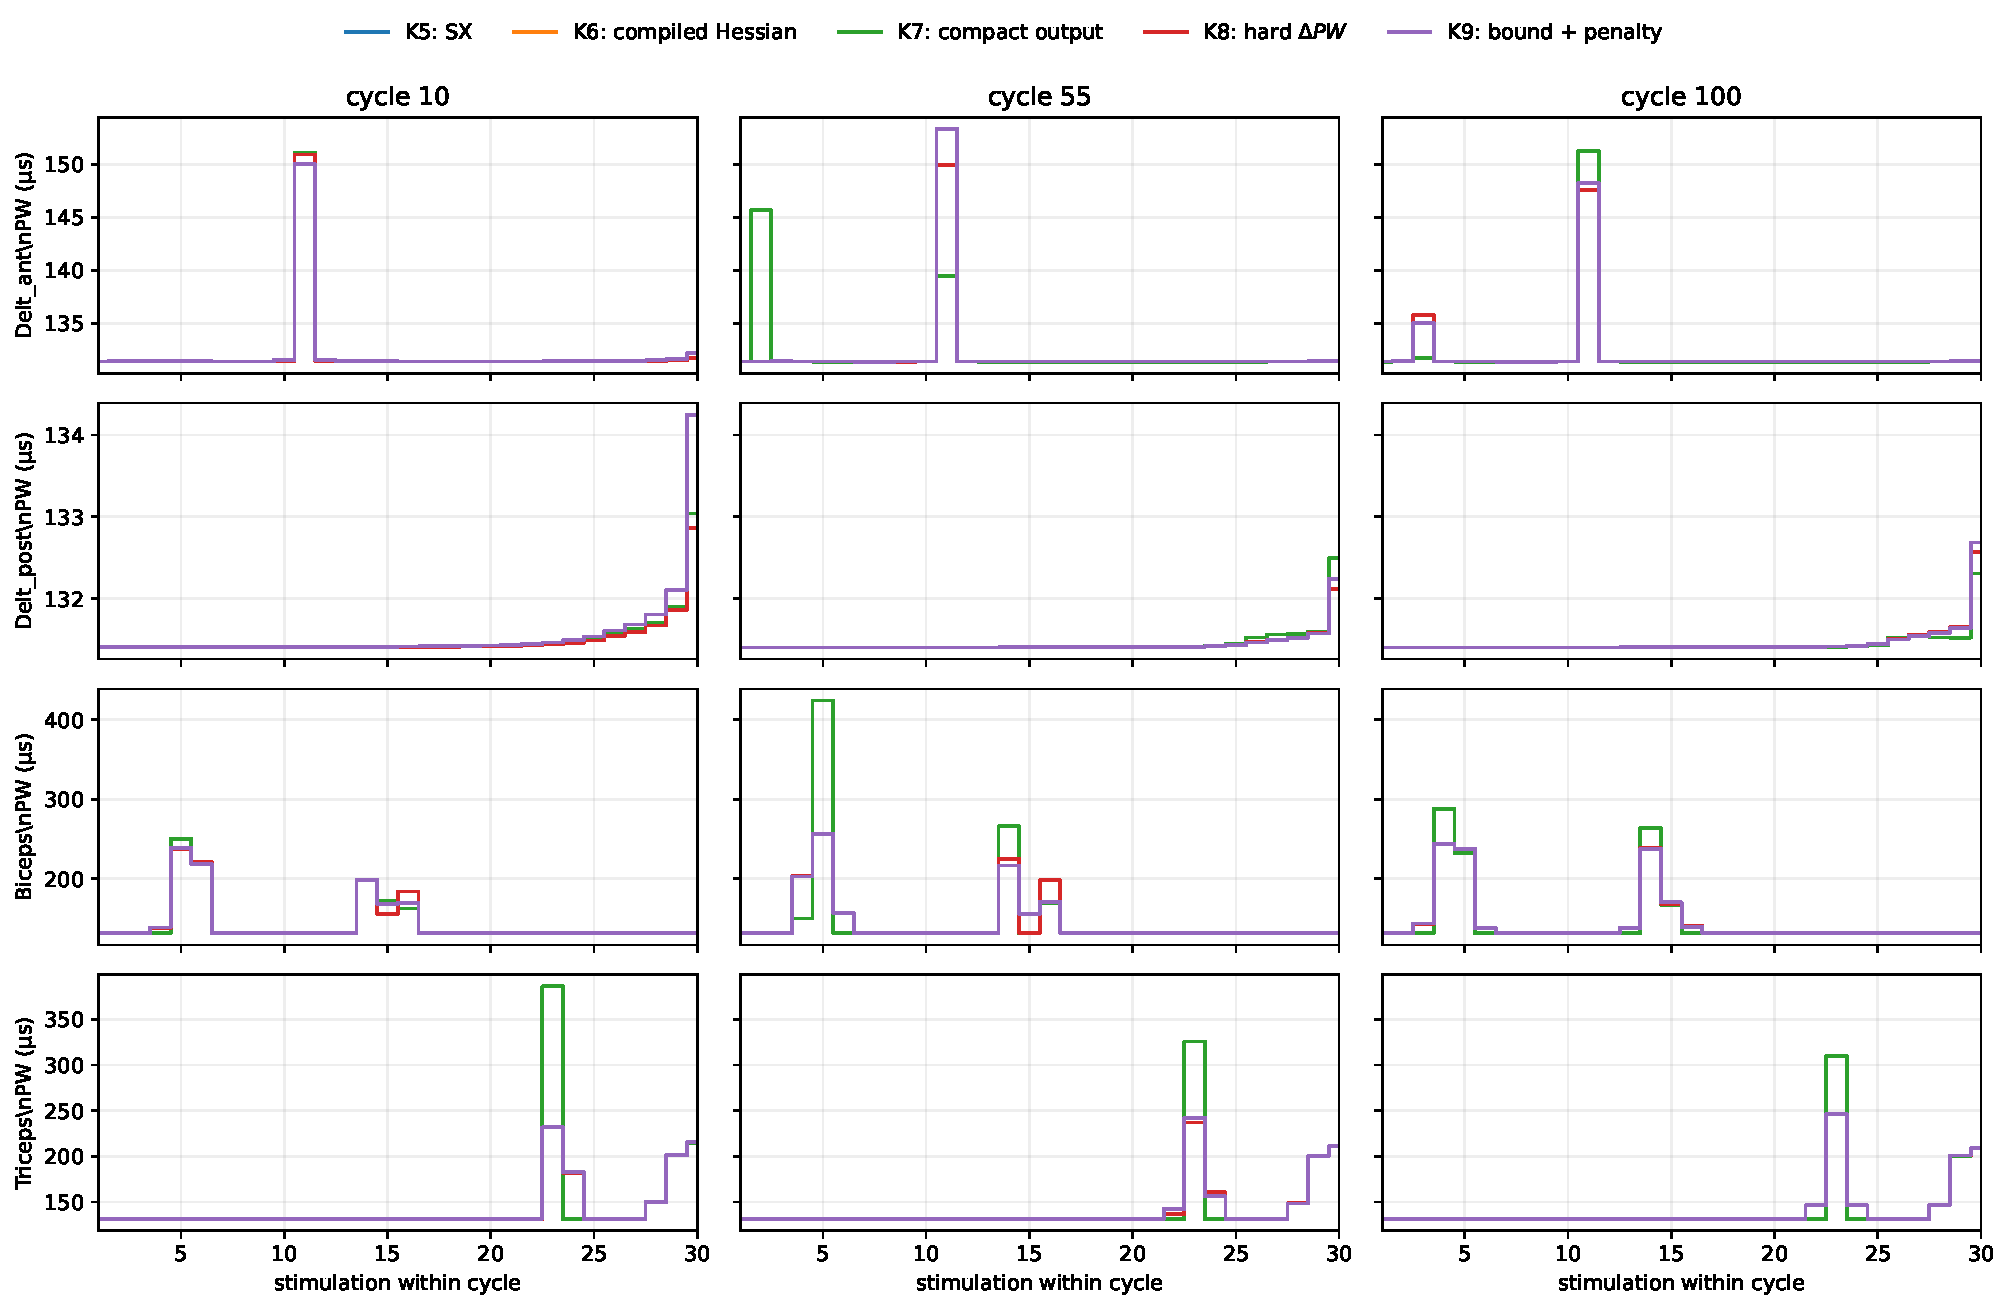
\includegraphics[width=\linewidth]{figures/pulse_width_patterns_k5_k9.pdf}
\caption{Applied four-muscle pulse-width patterns at cycles 10, 55, and 100 for the validated 30 Hz K5--K9 IPOPT/MA57 archives. Values are the archived applied pulse widths in microseconds; the sample index is the stimulation within the one-second crank cycle.}
\label{fig:pw-patterns}
\end{figure}

The source data and plotting rules are recorded in \texttt{scripts/plot\_pulse\_width\_patterns.py}. It fails when a trajectory does not retain all requested cycles or the expected four applied-pulse-width channels, preventing a partial archive from being compared silently.

\section{Frequency, periodic calcium, and solver checkpoints}

For a one-second crank cycle with $N_s$ evenly spaced pulses, periodic-node calcium uses $h=1/N_s$ and recalculates
\[
d=e^{-h/\tau_c}, \qquad C_n^*=\frac{dH_0(h)(h/\tau_c)}{1-d}.
\]
Therefore 33, 35, 40, and $50\Hz$ are fixed-frequency periodic-calcium experiments, not reuse of a $30\Hz$ calcium trace. They represent the steady periodic regime after warm-up. A genuine frequency switch requires phase-resampling controls and initializing calcium at the new fixed point, or explicitly simulating the transition.

\begin{longtable}{@{}p{0.16\textwidth}p{0.22\textwidth}p{0.12\textwidth}p{0.12\textwidth}p{0.12\textwidth}p{0.20\textwidth}@{}}
\toprule
Frequency and case & Solver & Validated cycles & Hot median (s) & Hot P90 (s) & Status\\
\midrule
\endhead
30 Hz K5 & MadNLP 0.10.1 + MA57 & 100/100 & 0.925 & 1.193 & Native valid comparator.\\
33 Hz K7 & IPOPT + MA57 & 100/100 & 0.558 & 0.681 & Valid; below one second.\\
35 Hz K5 & IPOPT + MA57 & 100/100 & 0.875 & 1.451 & Valid; tail exceeds one second.\\
35 Hz K5 & MadNLP 0.10.1 + MA57 & 100/100 & 1.148 & 1.399 & Valid but not real-time.\\
40 Hz K5 & IPOPT + MA57 & 100/100 & 1.043 & 1.319 & Valid; median exceeds one second.\\
40 Hz K5 & MadNLP 0.10.1 + MA57 & 0/100 & -- & -- & Native continuity tolerance failure.\\
50 Hz K10 & IPOPT + MA57 & 100/100 & 1.488 & 1.716 & Robustness point, not real-time.\\
\bottomrule
\end{longtable}

The 33 Hz K7 result is the conservative high-frequency reference: it preserves periodic calcium, passes the mechanical audit, and remains below one second at P90. The 50 Hz K10 result is robust but outside a one-second controller budget. IPOPT/MUMPS did not produce a native valid 100-cycle trajectory under an otherwise identical K3--K5 protocol, so no MA57-versus-MUMPS speed ratio is reported. MadNLP 0.10.1 uses MA57 through its compiled interface, but it was not faster than IPOPT/MA57 at 30--35 Hz.

\section{ACADOS and a decision-efficient validation policy}

ACADOS is not assigned an IPOPT-equivalent internal objective or timing interpretation. Its reduced-dynamics IRK route can complete 100 windows but has retained a between-node velocity excursion; it is therefore diagnostic rather than physically equivalent. Its local Ding reconstruction is near machine precision at the map level, but the 76-cycle stopping point prevents a 100-cycle performance claim.

An exhaustive product of frequencies, solvers, graph options, and regularizers is neither necessary nor informative. Use IPOPT/MA57 as the certified frequency reference. Advance frequency only after feasibility passes. Test an independent solver at 30 Hz, at the last IPOPT point whose P90 is below one second, and at the first point beyond this threshold. Test MUMPS only as a controlled IPOPT linear-solver A/B. Retain ACADOS only after common DOP853 replay passes. Final rankings must report DOP853 objective, speed excursion, phase/work error, and pulse-width feasibility separately from native solver timings.

\section{Runtime reductions outside the nonlinear optimization}

NLP time is not the total controller latency. The following engineering measures reduce work outside optimization and must be reported separately from iteration time.

\begin{longtable}{@{}p{0.31\textwidth}p{0.33\textwidth}p{0.30\textwidth}@{}}
\toprule
Change & What it removes & Scientific safeguard\\
\midrule
\endhead
Offline reduced-profile construction and cache & Repeated full Biorbd/contact evaluation during each NLP call & Regenerate and audit after every biomechanical-model change.\\
Persistent RHO workers & Rebuilding Python/CasADi/IPOPT objects each cycle & Retain native transfer and certify every window.\\
Process isolation & Unsafe shared IPOPT/MA57/CasADi threaded state & IPC barrier before applying an adaptive block.\\
Compact RHO output and bounded history & Retention of unnecessary solution/model graphs & Preserve per-window audits and terminal state.\\
Warm starts and transferred bounds & Cold-start iterations & Apply the same seed and transfer rule to every solver comparison.\\
Blockwise weight updates & Cost reconstruction every cycle & Update only after both arms are certified; report boundary overhead.\\
\bottomrule
\end{longtable}

The paced two-arm campaign at $0.3\,$N\,m had a median pair wall time of 1.447 s, P90 of 2.412 s, and P95 of 5.673 s. The upper tail is dominated by ten-cycle boundaries where objectives are rewritten; it is part of the controller budget and must not be hidden by quoting only IPOPT internal solve time.

\section{External wheel moments}

The historical load is a global external moment $M=e_z\tau_e$ applied to the wheel segment. Its mechanically equivalent generalized load is
\[
Q_e(q)=J_{\omega,\mathrm{wheel}}(q)^T e_z\tau_e.
\]
In the unilateral model the wheel is downstream of shoulder, elbow, and crank rotation, so this resistance loads all three generalized coordinates. A torque applied internally at the crank bearing is a distinct model and can act only on the relative crank coordinate. The reduced equation must use $\eta_e(\theta)=q'(\theta)^TJ_{\omega,\mathrm{wheel}}^Te_z$, not merely a crank-coordinate tangent component. A 100-state direct-dynamics audit of corrected full representations gave a maximum mismatch of $1.14\times10^{-13}$.

\section{References}
\begin{enumerate}[label={[\arabic*]},leftmargin=*]
\item J. Ding, A. S. Wexler, and S. A. Binder-Macleod. ``A predictive model of fatigue in human skeletal muscles.'' \emph{Journal of Applied Physiology}, 89(4):1322--1332, 2000. doi:10.1152/jappl.2000.89.4.1322.
\item J. Ding, A. S. Wexler, and S. A. Binder-Macleod. ``A mathematical model that predicts the force-frequency relationship of human skeletal muscle.'' \emph{Muscle \& Nerve}, 26(4):477--485, 2002. doi:10.1002/mus.10198.
\item J. Ding, A. S. Wexler, and S. A. Binder-Macleod. ``Mathematical models for fatigue minimization during functional electrical stimulation.'' \emph{Journal of Electromyography and Kinesiology}, 13(6):575--588, 2003. doi:10.1016/S1050-6411(03)00102-0.
\item E. Hairer and G. Wanner. \emph{Solving Ordinary Differential Equations II: Stiff and Differential-Algebraic Problems}. Springer, 2nd edition, 1996. doi:10.1007/978-3-642-05221-7.
\item E. Hairer and G. Wanner. ``Stiff differential equations solved by Radau methods.'' \emph{Journal of Computational and Applied Mathematics}, 111(1--2):93--111, 1999. doi:10.1016/S0377-0427(99)00134-X.
\item F. De Groote, A. L. Kinney, A. V. Rao, and B. J. Fregly. ``Evaluation of direct collocation optimal control problem formulations for solving the muscle redundancy problem.'' \emph{Annals of Biomedical Engineering}, 44(10):2922--2936, 2016. doi:10.1007/s10439-016-1591-9.
\item K. Co, P. Puchaud, F. Moissenet, and M. Begon. ``Maximizing Task Endurance through Muscle Fatigue Minimization with Consideration of Muscle Fatigability and Task Contribution: an in-Silico FES Study of Handcycling.'' Manuscript, 2026.
\end{enumerate}

\end{document}
